% !TEX encoding = UTF-8 Unicode
\documentclass[12pt]{article}
\usepackage{geometry}
\geometry{a4paper}
\usepackage[utf8]{inputenc}
\usepackage[francais]{babel}
\usepackage{enumerate}
\usepackage{array}
\usepackage{fancyhdr}
\usepackage{parskip}
\usepackage{xlop}
\usepackage{color}
\usepackage{graphicx}
\usepackage[colorlinks=true, urlcolor=blue, linkcolor=black]{hyperref}
\usepackage[T1]{fontenc}
\usepackage{listings}
\usepackage[colorinlistoftodos,prependcaption,textsize=tiny]{todonotes}

\renewcommand{\FrenchLabelItem}{\textbullet}
\renewcommand{\arraystretch}{1.5}
\newcolumntype{B}{>{\bfseries}c}
\frenchbsetup{ReduceListSpacing=false}
\setlength{\parsep}{\parskip}

%----------------------------------------------------------------------------------------
%	TITLE PAGE
%----------------------------------------------------------------------------------------

\newcommand{\titleAT}{\begingroup % Create the command for including the title page in the document
\newlength{\drop} % Command for generating a specific amount of whitespace
\drop=0.07\textheight % Define the command as 10% of the total text height

\rule{\textwidth}{1pt}\par % Thick horizontal line
\vspace{2pt}\vspace{-\baselineskip} % Whitespace between lines
\rule{\textwidth}{0.4pt}\par % Thin horizontal line

\vspace{\drop} % Whitespace between the top lines and title
\centering % Center all text
{\Huge VR6}\\ % Title

\vspace{\drop} % Whitespace between the title and short horizontal line
\rule{0.3\textwidth}{0.4pt}\par % Short horizontal line under the title
\vspace{\drop} % Whitespace between the thin horizontal line and the author name

{\large \textsc{Adan Häfliger, Jonathan Link \& Xavier Willemin}}\par % Author name

\bigskip
\bigskip

{\small \textsc{26 mai 2017}}\par % Date

\vfill % Whitespace

\begin{figure}[!h]
	\centering
	%\includegraphics[scale=.35]{Cover.jpg}
\end{figure}

\bigskip

\rule{\textwidth}{0.4pt}\par % Thin horizontal line
\vspace{2pt}\vspace{-\baselineskip} % Whitespace between lines
\rule{\textwidth}{1pt}\par % Thick horizontal line

\thispagestyle{empty}

\endgroup}

%----------------------------------------------------------------------------------------
%	END TITLE PAGE
%----------------------------------------------------------------------------------------

\begin{document}

\titleAT

\newpage

\tableofcontents

\newpage

\section{The game}
One player has 2 minutes to go from the start of the level to one of the 3 available finish platforms. A second player must do everything to slow the progression of the first player by triggering obstacles at distance through a tablet.

\section{The controllers}
\todo[inline]{TO COMPLETE}

\section{Applications}
We built two independent applications. One for each player. The two applications communicate through the internet network.

\subsection{Level (Host)}
One application handles the HTC VIVE controllers and displays the 3D world containing the game level.

\subsection{Minimap (Client)}
The second application can be run on a tablet and displays a top-view map of the level. Through this app the second player can see  player 1 location and is able to trigger the walls distantly.

\subsection{Wall obstacles}
There are two types of wall obstacles.

\begin{itemize}  
\item Wall which once up will automatically goes down after a fixed number of seconds.
\item Wall which once up can be destroy with the canons of the ship.
\end{itemize}

\section{Networking}
Here is the list of all the possible messages that can be exchanges between the host and the client.

\begin{itemize}  
\item GetBlocks 
\item Block
\item GetWallObstacles 
\item WallObstacles
\item GetWallObstaclesImage 
\item WallObstaclesImage
\item GetStartPlateforms 
\item StartPlateform
\item GetPlateforms 
\item Plateform
\item GetRobotPosition
\item RobotPosition
\item Start
\item TriggerWallObstacle
\item WallObstacleHasFinished
\item WallObstacleHasFinished
\item GameOver
\item Finish
\end{itemize}

Here is an example of the structure of one message. This is the one used to send the blocks to the mini map in order to reconstruct the level.

\begin{lstlisting}
public class BlockMessage : MessageBase {
	public Vector3 position;
	public Vector3 size;
	public string name;
	public string materialName;
}
\end{lstlisting}

\subsection{Some graphical details}
To make the game more dynamic and pleasant to play we added some little animations. The clouds are moving in the sky, the water is animated as well and the finish green platforms moves to add a little difficulty. There is also some distance fog to increase the depth perception. We also took some time to make sure the environment stays coherent in terms of colors and aesthetic when we downloaded the assets or created ours.  

\section{Video}
The video is available here: \todo[inline]{TO COMPLETE}

\newpage

\section{Images}
\begin{figure}[h]
   \caption{\label{étiquette} view from the cockpit designed by ourself}
   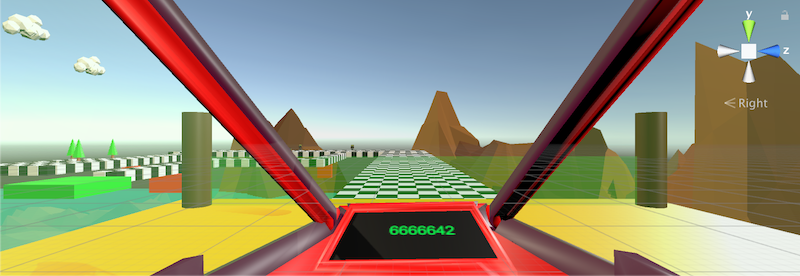
\includegraphics[scale=1]{images/cockpit.png}
\end{figure}

\begin{figure}[h]
   \caption{\label{étiquette} level 1 - low poly style}
   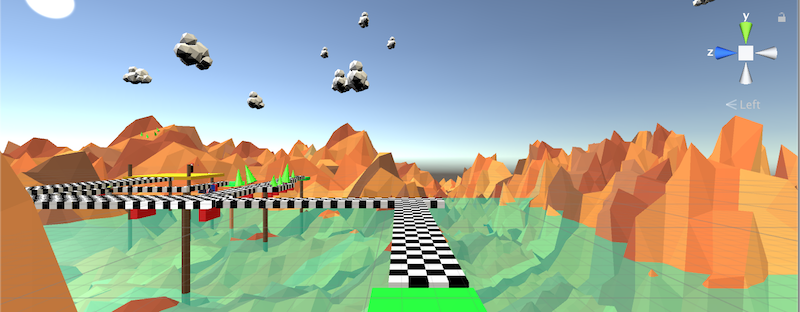
\includegraphics[scale=1]{images/level.png}
\end{figure}

\begin{figure}[!h]
   \caption{\label{étiquette} outside view of the ship piloted by player 1 with the htc vive}
   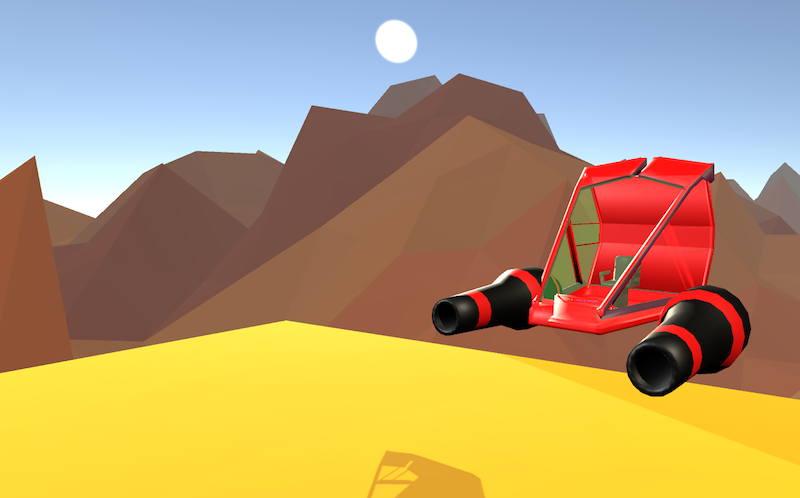
\includegraphics[scale=0.6]{images/ship.png}
\end{figure}

\begin{figure}[!h]
   \caption{\label{étiquette} top view of level 1 - the orange platform is the start and the green ones are different finishes}
   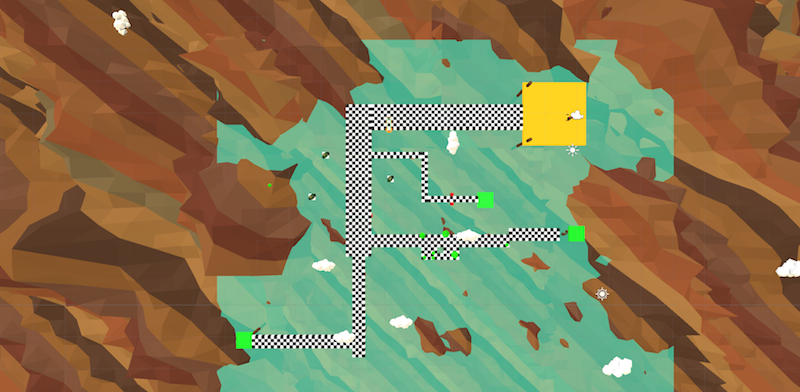
\includegraphics[scale=0.6]{images/topview.png}
\end{figure}

\begin{figure}[!h]
   \caption{\label{étiquette} a wall triggered by player 2 with the tablet}
   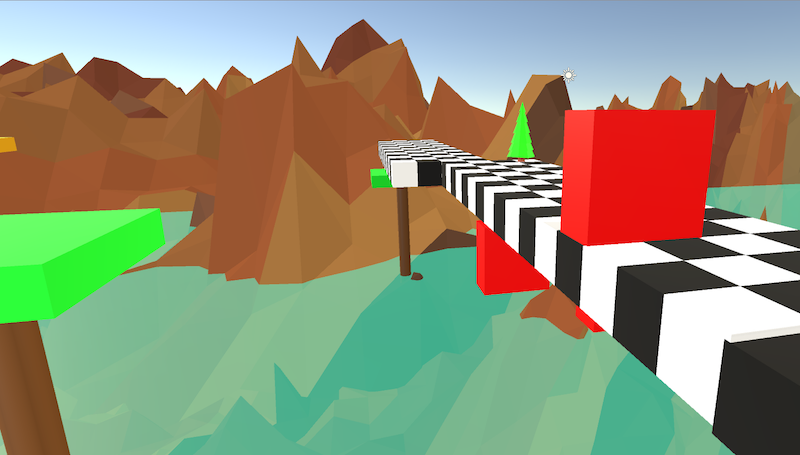
\includegraphics[scale=0.6]{images/wall.png}
\end{figure}


\end{document}
